\subsection{实验目的}
设计和使用低通滤波器,滤除分布在图像中的高斯白噪声。
\subsection{实验原理}
\subsubsection{高斯白噪声}
高斯白噪声是一种理想的噪声模型。高斯白噪声中,噪声振幅值是服从正态分布的。
\[ f(x)=\frac{1}{\sqrt{2\pi}\sigma}\mathrm{e}^{-\frac{(x-\mu)^2}{2\sigma^2}} \]
它的振幅分布直方图如下图\ref{fig:gwnhistogram}所示。
\begin{figure}[H]
	\centering
	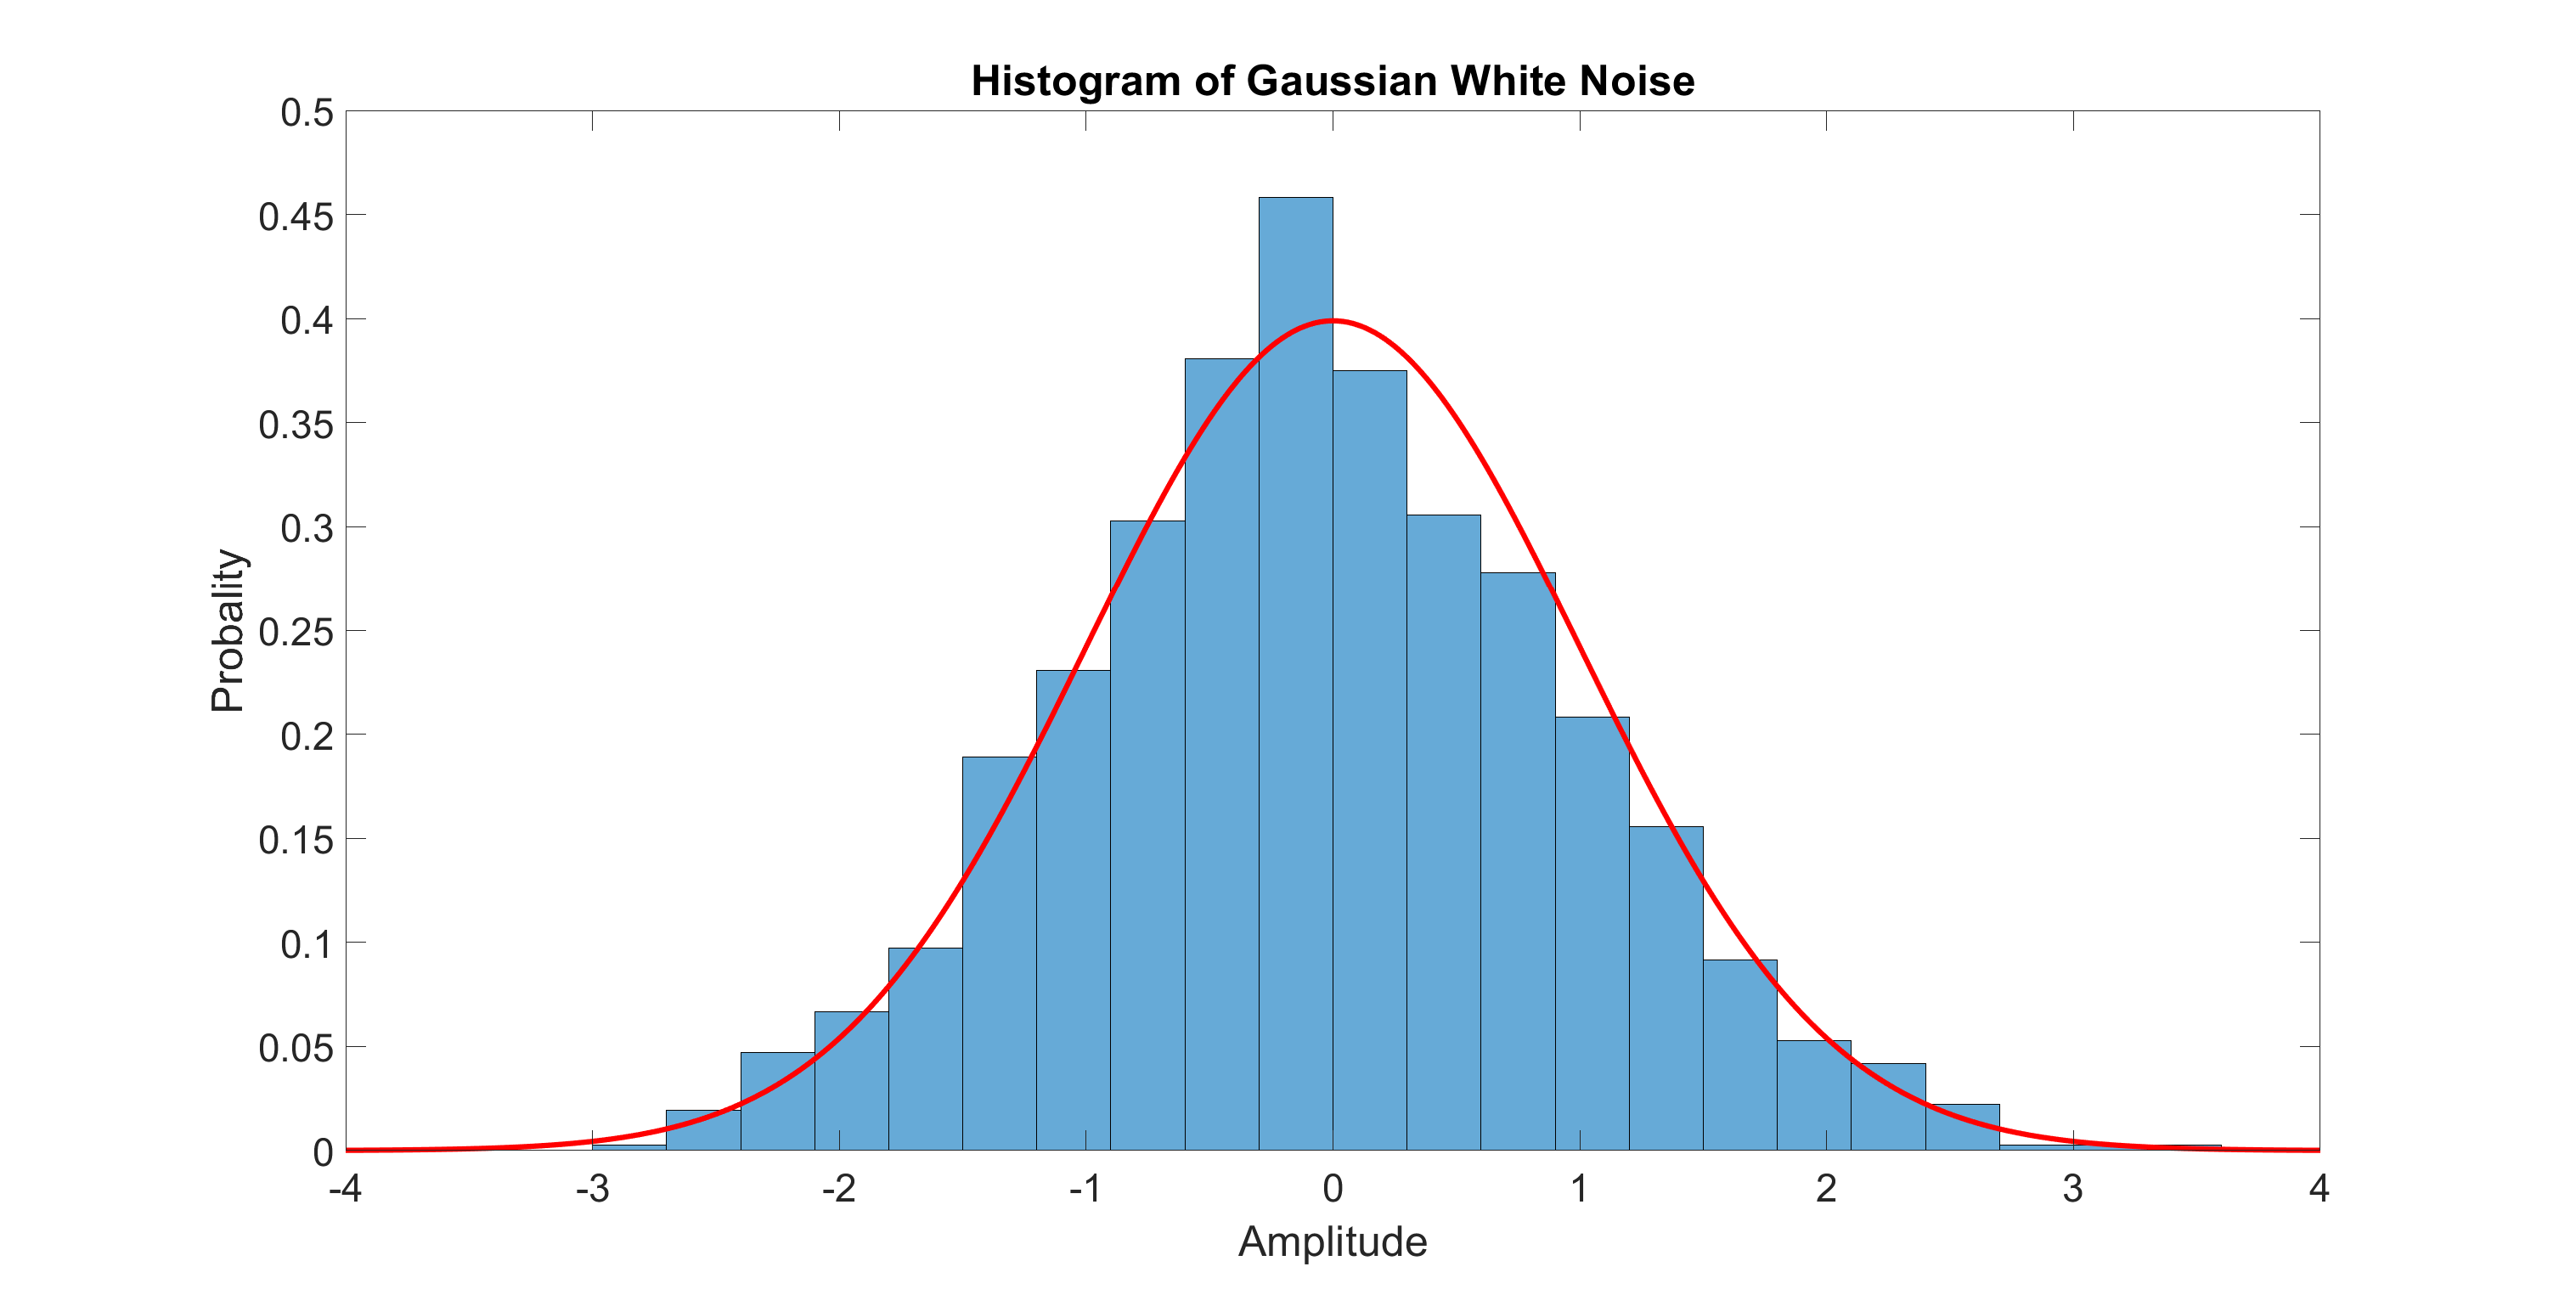
\includegraphics[width=0.7\linewidth]{figure/gwn_histogram}
	\caption{高斯白噪声幅度概率分布}
	\label{fig:gwnhistogram}
\end{figure}
它的功率谱是在频域内均匀分布的,在无限宽频带内满足
\[ G(\omega) = \frac{N_0}{2},\quad -\infty<\omega<+\infty \]
它的自相关函数为为
\[ R(\tau) = \frac{1}{2\pi}\int_{-\infty}^{+\infty}G(\omega)\mathrm{e}^{\mathrm{j}\omega t}\mathrm{d}\omega=\frac{N_0}{2}\delta(\tau) \]

在数字图像中,高斯白噪声线性叠加在图像中。设$f(x, y)$为原图像的表达式,$v(x, y)$为噪声在时空域上的表达式,则包含噪声的图像表达为
\[ g(x, y) = f(x, y) + v(x, y)\]
\subsubsection{傅里叶变换}
傅里叶变换是一种常用的信号分析方法。对于在时空上分布的二数字维图像$f(x, y)$,有傅里叶变换
\[ F(u, v) = \sum_{n = 0}^{N - 1}\sum_{m = 0}^{M - 1}\mathrm{e}^{-\mathrm{j}(\omega_kn+\omega_lm)}f(n, m) \]
\subsubsection{低通滤波器}
\subsection{实验流程}
\subsection{实验程序}
\subsection{实验结果和分析}